\documentclass[10pt]{beamer}
\beamertemplatenavigationsymbolsempty

\usepackage[utf8]{inputenc}
\usepackage{default}

\usepackage{graphicx}
\graphicspath{{pictures/}}

\usepackage[french]{babel}
\usepackage[T1]{fontenc}

\usetheme{metropolis}
%\usecolortheme{dove}

\begin{document}

\begin{frame}
\frametitle{Université de Technologie de Belfort-Montbéliard\\
            Département informatique}
\begin{center}
    {\LARGE Projet IN55}\\
    \vskip 1em
    {\Large Animation d'un personnage 3D}
\end{center}
\vskip 1em
\begin{flushright}
    Responsable: Fabrice Lauri
\end{flushright}
Florent \textsc{Jacquet}\\
Romain \textsc{Thibaud}\\
Antonin \textsc{WALTZ}\\
{\scriptsize IN55 - A15}
\end{frame}

\begin{frame}
 	\frametitle{Sommaire}
	\tableofcontents
\end{frame}

\section{Modélisation}
\begin{frame}
\frametitle{Modélisation}
\begin{itemize}
    \item Utilisation de Blender
    \item 3 animations : marcher, s'asseoir, voler
\end{itemize}
\begin{figure}[htpb]
    \centering
    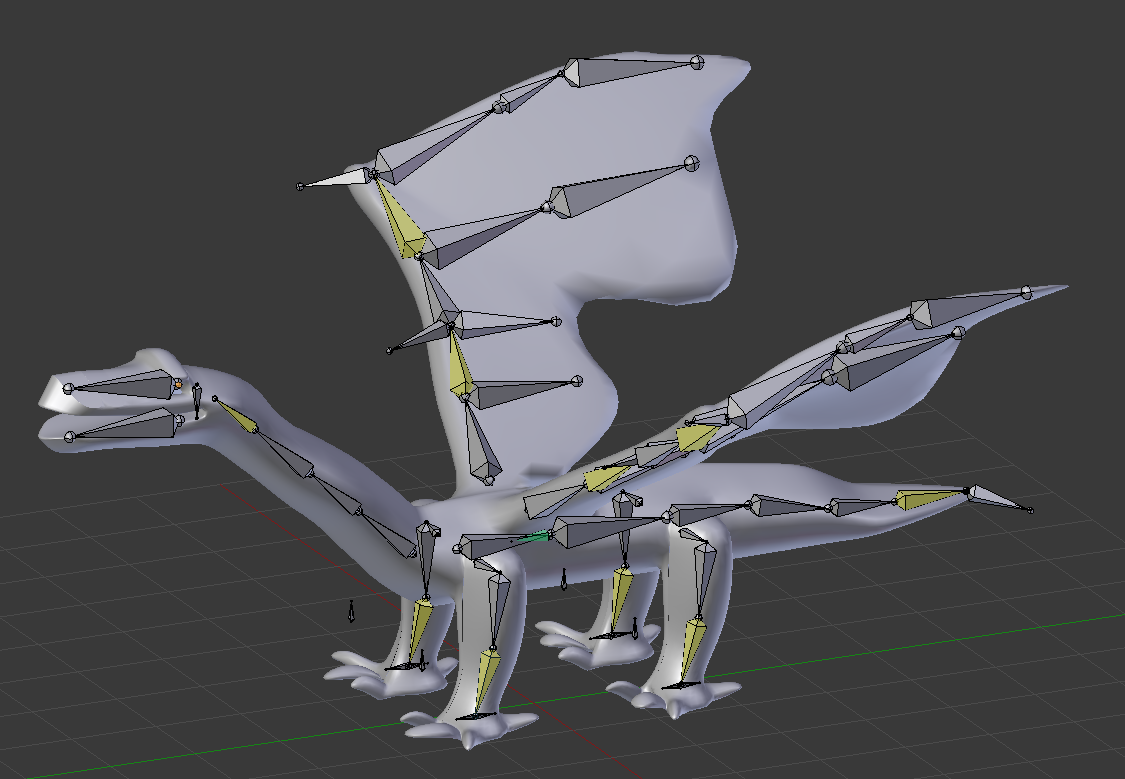
\includegraphics[width=0.7\linewidth]{armature.png}
    \caption{Modèle du dragon avec son armature}
\end{figure}
\end{frame}

\section{Architecture}
\begin{frame}
\frametitle{Structure d'un Mesh}
\begin{figure}[H]
    \begin{center}
        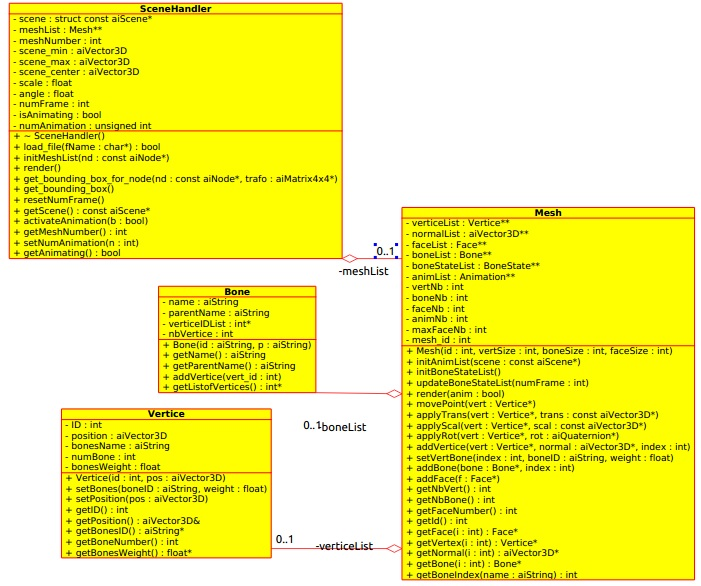
\includegraphics[width=0.8\textwidth]{MeshStructure.jpg}
        \caption{Diagramme de classe pour la structure d'un Mesh}
    \end{center}
\end{figure}
\end{frame}

\begin{frame}
\frametitle{Structure d'une Animation}
\begin{figure}[H]
    \begin{center}
        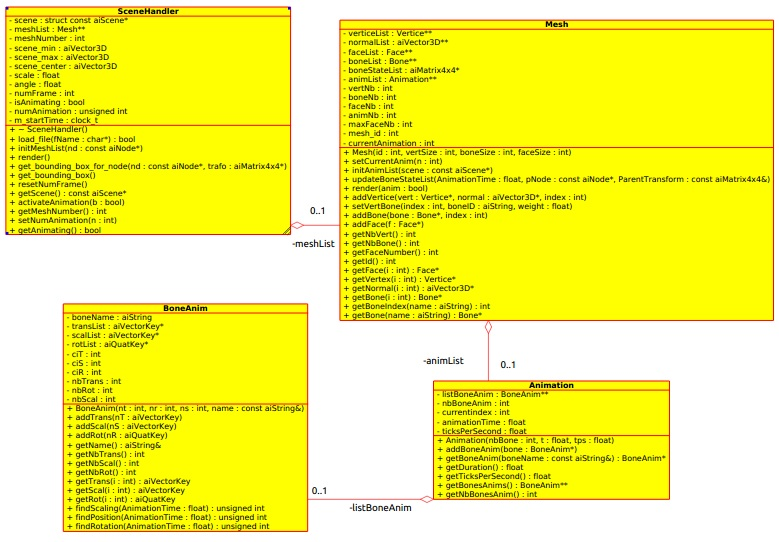
\includegraphics[width=0.9\textwidth]{AnimStructure.jpg}
        \caption{Diagramme de classe pour la structure d'une animation}
    \end{center}
\end{figure}
\end{frame}

\section{Animation}
\begin{frame}{Calcul des transformations}
    \begin{itemize}
        \item Utilisation d'une liste de matrices, associée aux bones
        \item La scène passe au shader les matrices de transformation du monde
        \item Le mesh passe au shader les informations pour chaque vertex (position, normale, bone ID, poids)
    \end{itemize}
\end{frame}

\begin{frame}{Shader}
    \begin{itemize}
        \item Entrées: Position, Normale, BoneTransform[4], Weights[4]
        \item Sorties: Normal, WorldPosition
        \item Entrées uniformes: ModelPosition, WorldTransform
    \end{itemize}
    Actions effectuées:
    \begin{itemize}
        \item Somme de toutes les transformations de BoneTransform multipliées par Weights.
        \item Multiplication de la transformation obtenue par celle du monde et du mesh
        \item Multiplication de cette dernière matrices par la position du vertex et la normale pour les envoyer en sortie
    \end{itemize}
\end{frame}

\section{Bilan}
\begin{frame}
\frametitle{Difficultés rencontrées}
\begin{itemize}
	\item Prise en main des Inverse Kinematics et de Blender en général
	\item Prise en main de la librairie Assimp
	\item Comprendre comment parcourir de grandes quantités de données à travers des structures complexes pleines de références croisées
	\item Gestion de la mémoire en C++
\end{itemize}
\end{frame}

\begin{frame}
\frametitle{Améliorations}
\begin{itemize}
	\item Texturer le modèle
	\item Intégrer un système de gestion de la lumière
	\item Améliorer la fluidité et le maniement de la caméra libre
\end{itemize}
\end{frame}

\begin{frame}
\begin{center}
\textbf{Merci de votre attention}\\
    Questions?\\
    Remarques?\\
\end{center}
\end{frame}

\end{document}
